%%-*-latex-*-

\documentclass[a4paper]{article}

\usepackage[francais]{babel}
\usepackage[OT1]{fontenc}
\usepackage[latin1]{inputenc}
\usepackage{amsfonts}

\usepackage{xspace}
\usepackage{amssymb,amsmath,stmaryrd}
\usepackage{graphicx}

/home/rinderkn/LaTeX/TeX/trace.tex
/home/rinderkn/LaTeX/TeX/commands.tex
/home/rinderkn/LaTeX/TeX/ocaml_syntax.tex

\title{Examen de programmation fonctionnelle en Objective Caml}
\author{Christian Rinderknecht}
\date{Mercredi 28 avril 2004}

\newcommand{\evalf}[2]{\llbracket{#1}\rrbracket{#2}}
\newcommand{\bitem}{\item[$\bullet$]}

\begin{document}

\maketitle

%\begin{center}
\centerline{\textbf{Dur�e: 2 heures. Documents et calculatrices ne sont
pas autoris�s.}}
%\end{center}


\section{Syntaxe et s�mantique}

\noindent Pour chacun des programmes suivants \textbf{dans l'ordre du sujet},

\begin{enumerate}

  \item construisez l'arbre correspondant (\textbf{� l'encre}),
 
  \item dans chaque arbre, reliez les variables dans les expressions �
  leur lieur (\textbf{dans une encre diff�rente}),

  \item identifiez les variables libres (\textbf{� l'encre dans
  l'arbre et dans une phrase}),

  \item d�crivez formellement son ex�cution � l'aide de la s�mantique
  suivante, o� $\evalf{e}{\rho}$ est la valeur de l'expression $e$
  dans l'environnement $\rho$:
\begin{align*}
\evalf{\overline{n}}{\rho} &= \dot{n} \ \ \textnormal{o� $\overline{n}$
  est un entier mini-ML et $\dot{n} \in \mathbb{N}$}\\
\evalf{e_1 \texttt{+} \, e_2}{\rho} &= \evalf{e_1}{\rho} +
\evalf{e_2}{\rho} \ \ \textnormal{etc.}\\ 
\evalf{\lpar{e}\rpar}{\rho} &= \evalf{e}{\rho}\\
\evalf{x}{\rho} &= \rho(x) \ \ \textnormal{(la premi�re liaison de $x$ dans $\rho$)}\\
\evalf{\Xfun \,\, x \rightarrow e}{\rho} &= \langle\Xfun \,\, x
\rightarrow e, \rho\rangle\\
\evalf{\Xlet \,\, x = e_1 \,\, \Xin \,\, e_2}{\rho} &= \evalf{e_2}{((x
  \mapsto \evalf{e_1}{\rho}) \oplus \rho)}\\
\evalf{e_1 \,\, e_2}{\rho} &= \evalf{e}{((x \mapsto \evalf{e_2}{\rho})
  \oplus \rho')} \ \ \textnormal{o�} \ \ \evalf{e_1}{\rho} = \langle\Xfun \,\, x
\rightarrow e,\rho'\rangle
\end{align*}
  L'�valuation consiste � appliquer les �quations de la gauche vers la
  droite jusqu'au r�sultat ou une impossibilit� (c.-�-d. erreur �
  l'ex�cution).

\end{enumerate}

\noindent \textbf{Programme 1}
\begin{verbatim}
let x = 1 in ((let x = 2 in x) + x);;
\end{verbatim}

\noindent \textbf{Programme 2}
\begin{verbatim}
fun y -> x + (fun x -> x) y;;
\end{verbatim}

\noindent \textbf{Programme 3}
\begin{verbatim}
let x = 1 in
  let f = fun y -> x + y in
  let x = 2
in f(x);;
\end{verbatim}

\noindent \textbf{Programme 4}
\begin{verbatim}
let x = 0 in
  let id = fun x -> x in
  let _ = let y = 2 in id (y) in
  let x = (fun x -> fun y -> x + y) 1 2
in x+1;;
\end{verbatim}

\noindent \textbf{Programme 5}

\begin{verbatim}
let compose = fun f -> fun g -> fun x -> f (g x) in
  let square = fun f -> compose f f in
  let double = fun x -> x + x in
  let quad = square double 
in square quad;;
\end{verbatim}


\section{Programmation}

\noindent Le type des arbres binaires est d�fini par:
\begin{verbatim}
type 'a arbre = Vide | Noeud of 'a * 'a arbre * 'a arbre
\end{verbatim}


\noindent Un arbre binaire de recherche est un arbre binaire tel que:

\begin{itemize}
  
  \bitem toutes les �tiquettes du sous-arbre de gauche
  (respectivement, de droite) sont inf�rieures (respectivement,
  sup�rieures) � l'�tiquette de la racine,

  \bitem r�cursivement, les deux sous-arbres sont eux-m�mes des arbres
  de recherche.

\end{itemize}

\begin{figure}[htbp]
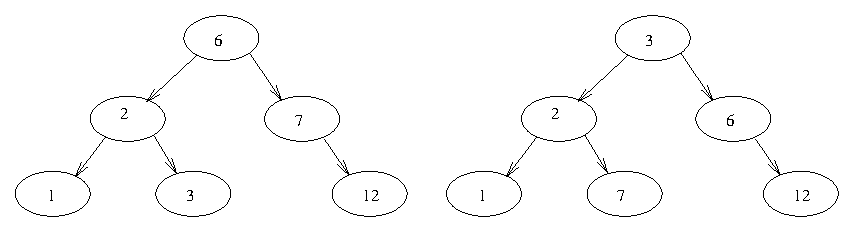
\includegraphics[width=320pt]{arech.eps}
\end{figure}

Le premier arbre ci-dessus est un arbre de recherche. Le second n'en
est pas un car~7 est plus grand que~3 mais il se trouve dans le
sous-arbre de gauche de la racine.

\begin{itemize}

  \bitem �crire une fonction \texttt{minimum} qui renvoie le plus
  petit �l�ment d'un arbre binaire de recherche. On d�clenchera
  l'exception \texttt{Not\_found} si l'arbre est vide.

  \bitem �crire une fonction \texttt{appartient} currify�e qui indique
  si une �tiquette donn�e appara�t dans un arbre de recherche
  donn�. On tirera parti du fait que l'arbre est class� pour que la
  recherche soit plus rapide que dans un arbre binaire quelconque.

  \bitem �crire une fonction \texttt{ajoute} qui ajoute un n{\oe}ud
  dans un arbre de recherche de fa�on � ce que celui-ci reste un arbre
  de recherche. Cela se fait en rajoutant une feuille � l'arbre.

\end{itemize}


\end{document}
